%! TEX root = main.tex
\section{Star formation and pre MS}\linkdest{starformation}

\begin{wordonframe}{da fare/ref}
\begin{itemize}
    \item SIS: shu 1977
    \item Rev Larson 2003: The physics of star formation
    \item Evans 1999 - Physical Conditions in Regions of Star Formation
    \item Bate 2011 - Collapse of a molecular cloud core to stellar densities: the formation and evolution of pre-stellar discs
    \item Onset of star formation: kippenhahn wiegert 248'-255' (131-134) -26.1: isothermal plane parallel and spherical object in HE
    \item Formation of protostars: kippenhahn wiegert 256'-265' (135-139)
    \item Star formation and early evolution: salaris cassisi 105' (119)
        \item Stahler chap 9: Cloud equilibrium and stability
\end{itemize}
\end{wordonframe}


\begin{frame}[allowframebreaks]{List of things}
%\printbibliography[keyword={inference},heading=beamer]
%\printbibliography[keyword={\mybibcat},heading=beamer]
%\listofkeywords
\listoftodos
\end{frame}

\subsection{Clouds Properties}

\begin{frame}{Clouds Zoology}
    \begin{columns}[T]
        \begin{column}{0.4\textwidth}
            \begin{itemize}
                \item Clouds: contains $80\%$ MW's $H_2$ (\num{2e9}$\msun{}$ in galactic disk): $3\%$ converted into stars, $\tau\approx\SI{3e7}{\year}$, MW's star formation rate now \SI{4}{\solarmass\per\year}
                    \item Collapse of dense core into protostars: Ambipolar diffusion, inside-out collapse, magnetized infall, Rotational effects
                \end{itemize}
        \end{column}
        \begin{column}{0.6\textwidth}
\begin{figure}[!ht]
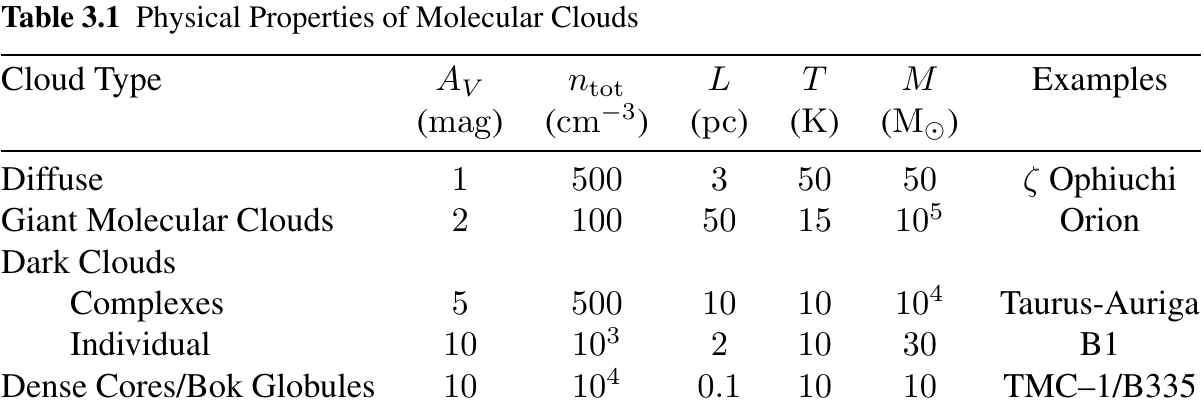
\includegraphics[trim={0cm 0cm 0cm 0cm},clip, keepaspectratio,width=0.8\textwidth]{cloudsprops}\label{fig:cloudsprops}
\end{figure}
        \end{column}
    \end{columns}
    \begin{itemize}
                    \item OB-association are correlated to giant molecular clouds: observations in \SI{2.6}{\milli\meter} of $^{12}C^{16}O$  - $^{13}C^{16}O$ lines to probe interior 
                    \item GMC are composed by clumps - clump (mass: \SI{250}{\solarmass},radius: \SI{1.5}{\parsec}, num dens: \SI{550}{\per\cubic\cm} ) - clump mass distro: $N=N_0(\frac{M}{M_{min}})^{-1.5}$, for $M>M_{min}\approx$\SI{30}{\solarmass}. Smallest entities: dense cores and Bok globules (harbour infrared sources: star formation).
                    \item Extended massive atomic H envelope: comparable mass of enclosed complex, several times its linear size. Observations: excess \SI{21}{\cm} line, $T\approx$\SIrange{50}{150}{\kelvin}.
                    \item Virial-T: $\frac{1}{2}\TtwoDy{t}{I}=2T+2U+W+M$ - moment of inertia $I=\int\rho|\vec{r}|^2\,d^3r$, total kin energy $T=\frac{1}{2}\int\rho|\vec{u}|^2\,d^3x$, total thermal energy $U=\frac{3}{2}\int nKT\,d^3x=\frac{3}{2}\int P\,d^3r$, gravitational potential energy $W=\frac{1}{2}\int\rho\phi_g\,d^3x$, Magnetic Energy $M=\frac{1}{8\pi}\int|\vec{B}|^2\,d^3x$.
        \end{itemize}
Free-fall time:
\begin{align*}
&R=L/2, W\approx-\frac{GM^2}{R}, \frac{1}{2}\TtwoDy{t}{I}\approx-\frac{GM^2}{R}\\
&I\approx MR^2\Rightarrow t_{ff}\approx(\frac{R^3}{GM})^{1/2}\approx\SI{7e6}{\year}(\frac{M}{\num{e5}\msun{}})^{-1/2}(\frac{R}{\SI{25}{\parsec}})^{3/2}\\
&\rho=\frac{M}{R^3}: t_{ff}\approx(\frac{3\pi}{32G\rho})^{-\frac{1}{2}}: \tau_{MC}\approx\tau_{ff}
\end{align*}
\end{frame}

\begin{frame}{Support of giant complexes: force balance $2T+2U+W+M=0$}
    \begin{itemize}
        \item Thermal pressure $U\approx \frac{MRT}{\mu}$: $\frac{U}{|W|}\approx \frac{MRT}{\mu}(\frac{GM^2}{R})^{-1}=\num{3e-3}(\frac{M}{\num{e5}\msun{}<++>})^{-1}(\frac{R}{\SI{25}{\parsec}})(\frac{T}{\SI{15}{\kelvin}})$ - Giant complexes not sustained by thermal pressure
        \item Magnetic field (Zeeman split of HI \SI{21}{\cm} or OH \SI{18}{\cm} lines): $\frac{M}{|W|}=\frac{|B|^2R^3}{6\pi}(\frac{GM^2}{R})^{-1}=0.3(\frac{B}{\SI{20}{\micro\gauss}})^2(\frac{R}{\SI{25}{\parsec}})^4$ - any selfgrav. mainly supported by ordered magneti field settles into planar config. BUT this is in contrast with obs. - random component of $\vec{B}$ coexistin with smooth background: MHD can provide isotropic support preventin flattening.
        \item Kin. ener. from random motion of clumps: $\frac{T}{|W|}=\frac{1}{2}M\Delta V^2(\frac{GM^2}{R})^{-1}=0.5(\frac{\Delta V}{\SI{4}{\kilo\meter\per\second}})^2(\frac{M}{\num{e5}\msun{}})^{-1}(\frac{R}{\SI{25}{\parsec}})$ - Rosetta line-of-sight dispersion is \SI{2.3}{\kilo\meter\per\second}, multiplied by $\sqrt{3}$ for random 3D velocity field, gives $\Delta V\approx V_{vir}=\sqrt{\frac{GM}{R}}$ (speed of gas parcel traversin cloud in $t_{ff}$).
        \item Line broadening: Thermal and bulk motion of emitting gas. Larson's law: $\Delta V=\Delta V_0(\frac{L}{L_0})^n$, $\Delta V_0\approx\SI{1}{\kilo\meter\per\second}$, $L_0=\SI{1}{\parsec}$, $n\approx0.5$
        \end{itemize}
\end{frame}

\begin{frame}{Birthline}
    \begin{columns}[T]
        \begin{column}{0.6\textwidth}
    \begin{itemize}
        \item Accreting stars: as gas falls onto star it lower potential energy onto the star $\Delta W\approx -\frac{GM_*\Delta m}{R}$, and gas brings its internal energy $\Delta U=\epsilon\frac{GM_*\Delta M}{R}$, $\epsilon=1$: all energy converted into heat, $\epsilon<1$: bound orbit, $\epsilon=0$: gas tot cold
        \item Birthline is locus in HDR of pre-MS stars with protostellar radius: surface L and $T_e$ are set by infalling dynamics, R is determined by internal structure
        \end{itemize}
        \end{column}
        \begin{column}{0.4\textwidth}
            \begin{align*}
                &\tkh{}=\frac{GM_*^2}{RL}: \dot{R}_*=-n_1 \frac{R_*}{\tkh{}}\\
                &L=4\piR_*^2\sigma T_e^4: \dot{L}_*=-n_2 \frac{L_*}{\tkh{}}\\
                &\Rightarrow\tkh{}\propto L_*^{-3/2}\tag{fixed mass}
            \end{align*}
        \end{column}
    \end{columns}
\end{frame}

\begin{frame}{Isothermal clouds: Density Structure}
    \begin{align*}
        &-\frac{1}{\rho}\nabla P-\nabla\phi_g=0, P=\rho a_T^2\Rightarrow \ln{\rho}+\frac{\phi_g}{a_T^2}=\const{}: \rho(r)=\rho_c\exp{-\frac{\phi_g}{a_T^2}}\tag{Spherical}\\
        &\nabla^2\phi_g=4\pi G\rho\Rightarrow \frac{1}{r^2}\TDof{r}(r^2\TDy{r}{\phi_g})=4\pi G\rho=4\pi G\rho_c\exp{-\frac{\phi_g}{a_T^2}}\\
        &\frac{1}{\xi^2}\TDof{\xi}(\xi^2\TDy{\xi}{\psi})=\exp{-\psi},\xi=\sqrt{\frac{4\pi G\rho_c}{a_T^2}}r,\psi=\frac{\phi_g}{a_T^2}\tag{isothermal Lane-Emden}\\
        &\psi(0)=0,\psi'(\xi)\xrightarrow{\xi\to0}0\tag{Boundary conditions}\\
        &\frac{\rho}{\rho_c}\to\frac{2}{\xi^2}\Rightarrow\psi=\ln{\frac{\xi^2}{2}}, \rho(r)=\frac{a_T^2}{2\pi Gr^2}\tag{SIS: not satisfy conditions at 0 - large distance}\\
        &\rho_0=\frac{P_0}{a_T^2},r_0=\frac{\xi_0}{\sqrt{\frac{4\pi G\rho_c}{a_T^2}}}\tag{Specifying $P_0$,$a_T$ - $\frac{\rho_c}{\rho_0}$ gives non-dim radius $\xi_0$}\\
        &M=4\pi\int_0^{r_0}\rho r^2\,dr=4\pi\rho_c(\frac{a_T^2}{4\pi G\rho_c})^{\frac{3}{2}}\int_0^{\xi_0}\exp{-\psi}\xi^2\,d\xi,m=\frac{P_0^{\frac{1}{2}}G^{\frac{3}{2}}M}{a_T^4}=(4\pi \frac{\rho_c}{\rho_0})^{-\frac{1}{2}}(\xi^2\TDy{\xi}{\psi})_{\xi_0}
        \end{align*}
        At beginning sequence $\frac{\rho_c}{\rho_0}=1$: $\xi_0=0$, $m=0$; with increasing density contrast m first rises to maximum $m_1=1.18$ at $\frac{\rho_c}{\rho_0}=14.1$, then decreses to minimum $m_2=0.695$, eventually approachin to $m_{\infty}=\sqrt{\frac{2}{\pi}}=0.798$: non dimensional mass of SIS.
    \end{frame}

    \begin{frame}{Gravitational stability of SIS}
        \begin{align*}
            &m=\frac{P_0^{\frac{1}{2}}G^{\frac{3}{2}}M}{a_T^4}: \xincreases{P_0},\xincreases{m}\Rightarrow\xincreases{\frac{\rho_c}{\rho_0}}(\xincreases{\xi_0})\Rightarrow \xincreases{P_c},\xincreases{\exv{P}}\tag{M fixed, $a_t$ fixed, low $\rho$ contrast, $\frac{\rho_c}{\rho_0}<14.1$}\\
            &M_{BE}=\frac{m_1a_T^4}{P_0^{\frac{1}{2}}G^{\frac{3}{2}}}\tag{For $\frac{\rho_c}{\rho_0}>14.1$ instability - critical value $M_{BE}$ where fundamental modes becomes unstab.}\\
            &\psi(\xi)=\exp{-\psi}\approx1-\frac{\xi_0^2}{6}\tag{Small $\xi$: $\psi(\xi)=\frac{\xi^2}{6}+O(\xi^4)$ - Density contrast for cloud of nonDim radius $\xi_0$}\\
            &m=(4\pi \frac{\rho_c}{\rho_0})^{-\frac{1}{2}}(\xi^2\TDy{\xi}{\psi})_{\xi_0}: M\approx \frac{\xi_0^3}{6\pi^{\frac{3}{2}}}\frac{a_T^4}{P_0^{\frac{1}{2}}G^{\frac{3}{2}}}\tag{DenseCore, BokGlobule are on edge of g.i.}\\
            &\xi=\sqrt{\frac{4\pi G\rho_c}{a_T^2}}r,\xi_0=\sqrt{\frac{4\pi G\rho_c}{a_T^2}}r_0: \xi_0^3=(4\pi)^{\frac{3}{2}}(\frac{\rho_c}{\rho_0})^{\frac{3}{2}}\frac{P_0^{\frac{3}{2}}G^{\frac{3}{2}}}{a_T^6}\tag{$\frac{\rho_c}{\rho_0}\approx1$}\\
            &\Rightarrow r_0^3\approx\frac{3Ma_T^2}{4\pi P_0},\xdecreases{r_0},\xincreases{P_0},P_0\frac{4\pi r_0^3}{3}\approx\const{}\tag{Boyle's law}\\
            &\rho(x,t)=\rho_0+\delta\exp{i(kx-\omega t)},\rho \frac{D\vec{u}}{Dt}=\rho[\TDy{t}{\vec{u}}+\scap{u}{\nabla}\vec{u}]=-\nabla P-\rho\nabla\phi_g\tag{stability against linear perturb}\\
            &-i\omega\delta\rho+ik\rho_0\delta u=0\tag{cont}\\
            &\delta P=\delta\rho a_T^2\tag{EOS}\\
            &-k^2\delta\phi_g=4\pi G\delta\rho\tag{Poiss.}\\
            &-i\omega\rho_0\delta u=-ik\delta P-ik\rho_0\delta\phi_g\tag{EOM}\\
            &\Rightarrow-\omega^2\delta\rho=-k^2\delta P-k^2\rho_0\delta\phi_g=-k^2a_T^2\delta\rho-k^2\rho_0\delta\phi_g\Rightarrow\omega^2=k^2a_T^2-4\pi G\rho_0\tag{dispersion relation}\\
            &\lambda_J=\sqrt{\frac{\pi a_T^2}{G\rho_0}}=\SI{0.19}{\parsec}\sqrt{\frac{T}{\SI{10}{\kelvin}}}(\frac{n_{H_2}}{\SI{e4}{\per\cubic\cm}})^{-\frac{1}{2}}, M_{BE}=M_J=\frac{m_1a_T^3}{\rho_0^{\frac{1}{2}}G^{\frac{3}{2}}}=1\msun{}(\frac{T}{\SI{10}{\kelvin}})^{\frac{3}{2}}(\frac{n_{H_2}}{\SI{e4}{\per\cubic\cm}})^{-\frac{1}{2}}
        \end{align*}
        Perturbation with $\lambda>\lambda_J$ grow exponentially: uniform sphere of diameter $\lambda_J$ has mass $2M_{BE}$.
    \end{frame}

\subsection{From clouds to proto-stars}\linkdest{protostellar}

\begin{frame}{Molecular Clouds: density and clumps formation}
\begin{itemize}
        \item Calculations: small fraction of collapsing cloud core attains density to form a star; in SIS model envelope is at rest instead of falling at approx twice $c_s$ as in dynamical collapse.
\item clouds equilibrium shape: Observed cloud mass greater than Jeans mass; Rotation and magnetic field support increases Jeans mass
\item $H_2$ molecules formation: dust grains enhance $H_2$ formation which increases with density and column density of at least $20\msun{}\si{\per\square\parsec}$ (Column density: Mangum shirley 2015) is required to shield from UV, where typical column density is $100\msun\si{\per\square\parsec}$ (Elmegreen 85, 93); column density of cold $H_2$ is hard to measure directly infact is measured indirectly by collisional excitation of other molecules and by relative decrese of 21-cm emission/absorption line strenght from deplition of atomic H. ($\msun/pc^2\approx 2*10^{-4}gr/cm^2$).
\item Collisional excitation cooling by molecular/atomic lines emission increases with density while external heating decreases: MC are very cold (\SIrange{10}{20}{\kelvin}); far IR emission of CO; in densest regions gas is thermally coupled to dust mantaining $T\approx10K$.
\item Inefficient conversion of MC into stars: turbulence, magnetic fields.
\item Almost all MC are star forming: short lifetime, young age - $\tau_{MC}$ approx crossing time of internal turbulent motion $<\SI{1}{\mega\year}$
\item Fragmentation. Youngest stars are in denser part of MC: denser clumps may originate from Small fluctuation amplified by gravitational instabilities or Supersonic turbulent motion may compress gas into observed clumpy structure.
\item How collapse is initiated - Prestellar cloud core: Gravitational instability, for example Bonnor-Ebert sphere that slightly exceeds stability threshold, or if prestellar core are magnetically supported condensing gradually by ambipolar diffusion (neutral species collapse) whereby gas contract slowly along across field lines (SIS: singular isothermal sphere with no magnetic support $\rho(r)=\frac{c_s^2}{2\pi Gr^2}$, $M(r)=\frac{2c_s^2}{G}r$).
\end{itemize}
\end{frame}

\begin{frame}{Inside-out Spherical collapse: formation and accretion onto protostar} 
    \begin{itemize}
        \item Equilibrium model with margin-stable $M_{BE}=\frac{1.18a_T^4}{\sqrt{P_O}G^{\frac{3}{2}}}$. Transition to ff collapse $V_{ff}\approx a_T$, ie $\frac{G\dot{M}t}{R_{ff}}\approx a_T^2$, $\dot{R}_{ff}\approx \frac{R}{t}$; for $\dot{M}>0$: $\dot{R}_{ff}>0$, region of ff spreads.
        \item At low $\rho$: \xaumenta{\rho} \xdiminuisce{T} (increases atomic/molecular lines cooling); At higher $\rho$: gas becomes thermally coupled to dust which controls T with its thermal emission - T is \SIrange{6}{12}{\kelvin} while $\rho$ spans many OM as long as core remains optically thin to dust thermal radiation ($n_{H_2}<\SI{e10}{\per\cubic\cm}$).
        \item Most collapse calculation assume early stages isothermal at \SI{10}{\kelvin} (whitworth 98) and a universal result of isothermal collapse is runaway growth of central density peak (Penston 66, Bodenheimer Sweigart 68, Larson 69)
        \item In absence of pressure gradient the collapse of uniform sphere happens in $t_{ff}\approx\sqrt{\frac{3\pi}{32G\rho}}$: denser inner regions collapse faster (Larson 73, Tohline 82). Numerics show that $\rho\propto r\expy{-2}$ for collapsing isothermal sphere asymptotically for smaller radii as long as isothermal approx holds (Larson 69, Ogino 99); peak width at any stage of order of Jeans length $\propto\rho\expy{-1/2}$.
        \item Rotation. Forming cloud core rotate as expected due to turbulence in MC (Burket Bodenheimer 00) - ''Angular Momentum Problem'': much more angular momentum in MC than rotating stars - magnetic field can't dispose excess angular momentum: formation of multiple system. Narita 84: competition between pressure and gravity near center - centrifugal force never become strong enough there to halt condensation (rather the material with higher angular momentum produce a disk). Also for SIS model rotation could produce disk then spiral density fluctuation could cause inward mass transfer or disk fragmentation.
        \item Collapse with Magnetic Field. Timescale Ambipolar Diffusion \SI{e7}{\year} which is one OM greater then ff timescale; as in the central part gravity force become dominant the core becomes more flattened along field lines, when central part becomes unstable runaway collapse begins (flattened, collapse speed approx sound speed). Ambipolar Diffusion may solve ''Magnetic flux problem'' for star formation

    \end{itemize}
\end{frame}

\frameinlbftrue
\begin{frame}{Optically Thick Phase}
    \begin{itemize}
        \item Always central density peak is realize in spite of thermal pressure never being negligible near central regions; spherical symmetry at later stage when optical depth of central regions becomes large and radiative cooling unimportant and T rises (3D calculation partially support spherical Approx: Bate 98): rotational flattening may eventually becomes important and transient spiral appears (gravitational torque transfer enough angular momntum outward to allow growth of central mass.
            \item Calculation show formation of central object or protostar: Larson 69, 72, Appenzeller Tscharnuter 75, Winkler Newman 80, Masunaga Inutsuka 00 (later stages), Wuchterl Tscharnuter 03.
            \item Central regions becomes opaque for thermal radiation of dust for $\rho_c>\SI{e-13}{\gram\per\cubic\cm}$ ($\num{2e10} H_2$ \si{\per\cubic\cm}), transition to adiabatic evolution: completely adiabatic for $\rho>\SI{e-12}{\gram\per\cubic\cm}$ with ratio of specific heat $\gamma=\frac{7}{5}$ consistent for $H_2$ gas. As density continues to rise pressure increses faster than gravity and collapse halts at $\rho_c\approx\SI{2e-10}{\gram\per\cubic\cm}$: first hydrostatic core is formed with accreting shock at surface (mass $0.01 \msun{}$, radius several AU); its properties are almost indep. of initial conditions/boundary conditions due to convergence toward selfsimilar behaviour during isothermal collapse.
            \item Formation of second hydrostatic core, mass $0.001\msun{}$, radius $\rsun{}$: when $T_c>\SI{2000}{\kelvin}$ $H_2$ dissociates reducing $\gamma<\frac{4}{3}$ required for stability, hence we have a second collapse phase producing runaway central concentration; rapid collapse is halted when H is completely ionized at center and $\gamma=\frac{5}{3}$. Second hydrostatic core bounded by accretion shock.
            \item Predicted stars begins its life as small embryo $<\num{e-2}\msun{}$, the accreting surface is surrounded by optically thick materials hence the shock is adiabatic: outer layers of protostars are strongly heated and expands rapidly, until the reach $4\rsun{}$ when acreted all materials of first hydrostatic core (Masunaga Inutsuka 00).
            \item When rotation is present materials from first hydrostatic core has significant angular momentum and sets into disk (Yorke Bodenheimer 99), outward angular momentum transfer is needed to have predicted accretion rate (Mercer Smith 84).
    \end{itemize}
\end{frame}
\frameinlbffalse

\begin{frame}{Onset of cloud formation ($\tau_{ff}\gg\tau{KH}$). Jeans Criterion}
\begin{columns}[T]
\begin{column}{0.55\textwidth}
    \begin{itemize}
        \item Infinite homogeneous gas at rest: not well defined state, ie for symmetry reasons also g. potential $\phi$ must be const but from Poiss. we have $\nabla^2\phi=4\pi G\rho$ hence $\rho=0$; but if we apply periodic perturb. of suff. small wavelength the single perturbation will behave like one with same $\lambda$ in isothermal sphere at static equilibrium
        \item Gas obeys to:
\begin{align*}
    &\PDy{t}{\vec{v}}+(\vec{v}\cdot\nabla)\vec{v}=-\frac{1}{\rho}\nabla P-\nabla\phi\tag{EOM/Euler}\\
    &\PDy{t}{\rho}+\vec{v}\cdot\nabla\rho+\rho\nabla\cdot\vec{v}=0\tag{cont. eq.}\\
    &\nabla^2\phi=4\pi G\rho,\ P=\frac{R}{\mu}\rho T=v_s^2\rho\tag{Poiss.}\\
    &P=\frac{R}{\mu}\rho T=v_s^2\rho\tag{EOS}
\end{align*} 
$T=T_0=\const$, $\rho=\rho_0=\const$, $\nabla^2\phi_0=4\pi G\rho_0$
    \end{itemize}
\end{column}
\begin{column}{0.45\textwidth}
    \begin{itemize}
        \item Perturbazioni:
\begin{align*}
    &\rho=\rho_0+\rho_1,P=P_0+P_1,\phi=\phi_0+\phi_1,\vec{v}=\vec{v}_1\\
&\PDy{t}{\vec{v}_1}=-\nabla(\phi_1+v_s^2\frac{\rho_1}{\rho_0})\\
&\PDy{t}{\rho_1}+\rho_0\nabla\cdot\vec{v}_1=0\\
&\nabla\phi_1=4\pi G\rho_1
\end{align*}
Homogeneous ODE system with constant coeffs.
\item Assuming isothermal pertur. ($v_s$ unperturbed) and taking only linear terms
\item Solutions prop.to $\exp{i(kx+\omega t)}$: $\PDof{x}=ik$, $\PDof{y}=\PDof{z}=0$, $\PDof{t}=i\omega$
    \end{itemize}
\end{column}
\end{columns}
\begin{columns}[T]
	\begin{column}{0.3\textwidth}
		\begin{align*}
		&\omega v_1+\frac{kv_s^2\rho_1}{\rho_0}+k\phi_1=0\\
		&k\rho_0v_1+\omega\rho_1=0\\
		&4\pi G\rho_1+k^2\phi=0
		\end{align*}
	\end{column}
	\begin{column}{0.3\textwidth}
Non trivial solution
		\begin{align*}
		&\begin{vmatrix}
            \omega&\frac{kv_s^2}{\rho_0}&k\\
		k\rho_0&\omega&0\\
		0&4\pi G&k^2\\
		\end{vmatrix}=0\\
		&\omega^2=k^2v_s^2-4\pi G\rho_0
		\end{align*}
	\end{column}
	\begin{column}{0.4\textwidth}
$k$ large: $\omega$ real (oscillations). 
\begin{align*}
    &\lambda<\lambda_J=\frac{2\pi}{k_J}=\sqrt{\frac{\pi}{G\rho_0}}v_s\tag{Stable}\\
    &k<k_J=\frac{4\pi G\rho_0}{v_s^2}\tag{Unstable}
\end{align*}
\end{column}
\end{columns}
Collapsing plane-parallel slab: $i\omega\approx\sqrt{G\rho_0}$
\end{frame}

\begin{frame}{Jeans inst ability in isothermal sphere}
    \begin{columns}[T]
        \begin{column}{0.5\textwidth}
            \begin{itemize}
                \item $P*>0$: we get the structure fro ma solution of LE equation for isothermal polytrope
                \item Virial T: Internal energy $E_i=c_VMT$, for g. energy $E_g=\Theta \frac{GM^2}{R}$ ($\Theta$ can be obtained from LE iqu.)
                \item Using  virial t. $\zeta E_i+E_h=4\pi R^3P_0$: per $\zeta=2$ si ha $P_0=\frac{c_VMT}{2\pi R^3}-\frac{\Theta GM^2}{4\pi R^4}$
                \item For small $R$ $P_0<0$, changes sign for increasing $R$, $P_0\to0$ for $R\to\infty$ and reaches a max. at $R_m$
                \item Differentiating eq for $P_0$ we found $R_M=\frac{4\Theta}{9}\frac{G\mu M}{RT}$
            \end{itemize}
        \end{column}
        \begin{column}{0.5\textwidth}
            \begin{itemize}
                \item Stab ility of LE solution - Starting at equilibrium at $P^*=P_0$: for $R<R_m$ (unstable config.) equilibrium pressure $P_0$ decreses with decreasing $R$, therefore after slight compression $P^*>P_0$ and sphere compress more, for $R>R_m$ $P_0$ (stable)increses during slight compression and sphere will expand back to equilibrium.
                \item Same as Jeans Stability crit.: $M=\frac{4\pi}{3}r_m^3\bar{\rho}$. $R_m^2=\frac{27}{16\pi\Theta}\frac{RT}{G\mu\bar{\rho}}$ where $R_m$ is critical radius of gas with mean density $\bar{\rho}$ and T which is marg. stable - comparing with critical Jeans wavelength, $\lambda_J=\sqrt{\frac{\pi} {G\rho_0}}v_s$: they are same OoM.
            \end{itemize}
        \end{column}
    \end{columns}
    Expression for critical mass (Jeans mass): $M>M_J$ are unstable:
	\begin{align*} 
        &M_J=\frac{4\pi}{3}\exv{\rho}R_m^3:\ M_J=\frac{27}{16}\sqrt{\frac{3}{\pi}}(\frac{R}{\Theta G})^{\frac{3}{2}}(\frac{T}{\mu})^{\frac{3}{2}}(\frac{1}{\exv{\rho}})^{\frac{1}{2}}\tag{Virial/LE eq}\\
&M_J=\num{1.2e5}\msun{}(\frac{T}{\SI{100}{\kelvin}})^{\frac{3}{2}}(\frac{\rho}{\SI{e-24}{\gram\per\cubic\cm}})^{-\frac{1}{2}}\mu^{-\frac{3}{2}}\tag{pertub.}
	\end{align*}
\end{frame}

\begin{frame}{End of Fragmentation: Transition to adiabatic collapse.}
	Cooling processes: $E_g\approx\frac{GM^2}{R}$ has to be radiated at rate $A\approx\frac{GM^2}{R}(G\exv{\rho})^{\frac{1}{2}}\propto\frac{G^{\frac{3}{2}}M^{\frac{5}{2}}}{R^{\frac{5}{2}}}$; radiation emission as fraction f of radiation emitted from black body $B=4\pi f\sigma T^4R^2$
	\begin{columns}[T]
		\begin{column}{0.5\textwidth}
In isothermal collapse ($B\gg A$) $M_J\propto\rho^{-\frac{1}{2}}$ so as density increases the cloud undergoes ''sub collapses''.
		\end{column}
		\begin{column}{0.5\textwidth}
At end of isothermal collapse, when matter becomes opaque $A\approx B$, begins adiabatic collapse phase (approx thermal equilibrium):
 \begin{align*}
&\nad=\TDly{P}{T}_a=\frac{2}{5}\\
&T\propto P^{\frac{2}{5}}, P\propto\rho T:\ T\propto\rho^{\frac{2}{3}}\\
&M_J\propto T^{\frac{3}{2}}\rho^{-\frac{1}{2}}\propto\rho^{\frac{1}{2}}
 \end{align*}
		\end{column}
	\end{columns}
At end of fragmentation $M_J\approx0.02\msun{}\frac{T^{\frac{1}{4}}}{f^{\frac{1}{2}}}$
\end{frame}

\begin{frame}{Free-fall collapse of (h-)sphere. Collapse onto condensed object.}
$(\frac{g}{\nabla P})\propto\frac{M}{RT}\propto\frac{1}{R}$: collapse is more and more dominated by (g)ravitation (homologous contraction: $\frac{r}{r_0}$, $\frac{\dot{r}}{r_0}$ are same for all shell at given t)
\begin{align*}
&\ddot{r}=-\frac{Gm}{r^2}\Rightarrow\frac{1}{2}\dot{r}^2=\frac{4\pi r_0^3}{3r}G\rho_0+\const{}\\
&\frac{\dot{r}}{r}=-\sqrt{\frac{8\pi}{3}G\rho_0(\frac{r_0}{r}-1)},\cos^2{\zeta}=\frac{r}{r_0}\Rightarrow \zeta+\frac{1}{2}\sin{2\zeta}=\sqrt{\frac{8\pi G\rho_0}{3}}t
\end{align*}
When opacity gets bigger in central regions collaps stalls. $\dot{M}=4\pi r^2v\rho$ constant in space and time over central mass $M$ in HE: $\frac{2}{r}+\frac{1}{\rho}\TDy{r}{\rho}+\frac{1}{v}\TDy{r}{v}$, $v=v_{ff}=\sqrt{\frac{GM}{2r}}$ so $\frac{1}{\rho}\TDy{r}{\rho}=-\frac{3}{2r}$ ie $\rho(r)=\frac{\const{}}{r^{\frac{3}{2}}}$.

Radiation loss: $L_{accr}=\frac{1}{2}v_{ff}^2(R)\dot{M}=\frac{1}{4}\frac{GM}{R}\dot{M}$.

Collapse calculation:
\begin{align*}
&\PDy{}{}+4\pi r^2v\rho=0,\ \TDof{t}=\PDof{t}+v\PDof{r}\\
&\PDy{t}{v}+v\PDy{r}{v}+\frac{GM}{r^2}+\frac{1}{\rho}\PDy{r}{P}=0\tag{EOM}\\
&\PDy{t}{u}+P\PDof{t}(\frac{1}{\rho})+v[\PDy{r}{u}+P\PDof{r}(\frac{1}{\rho})]+\frac{1}{4\pi\rho r^2}\PDy{r}{l}=0,\ l=-\frac{16\pi acr^2}{3\kappa\rho}T^3\PDy{r}{T}
\end{align*}
\end{frame}

\begin{frame}{Optically thin phase and core formation}
\begin{columns}[T]
\begin{column}{0.55\textwidth}
\begin{itemize}
	\item Isothermal phase $T\approx\SI{10}{\kelvin}$ - when instability turns nonlinear contraction isn't homologous ($t_{ff}$ is smaller for inner shell: $\rho\propto r^{-2}$).
	\item Central region becomes opaque at $\rho\approx\SI{e-13}{\gram\per\cubic\cm}$: density increases causes adiabatic pressure increases until collapse stops.
	\item As M core increases and radius decreases v of infalling materials exeeds sound speed: shock region separating supersonic rain from hydrostatic core.
	\item Hydrostatic core: protostar - $\rho_e$, $v_e$ infalling matter then $P_i=\rho_ev_e^2=\rho_e\frac{GM}{2R}$ (momentum conservation: $P+\rho v^2$ is the same on both sides) 
\end{itemize}
\end{column}
\begin{column}{0.45\textwidth}
\begin{figure}[!ht]
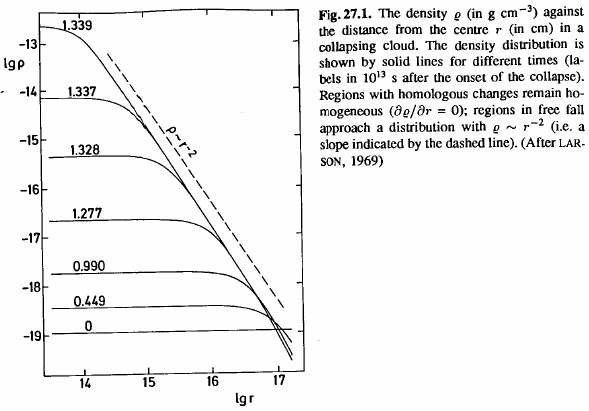
\includegraphics[trim={0cm 0cm 0cm 0cm},clip, keepaspectratio,width=0.8\textwidth]{collapsingdensity}\label{fig:collapsingdensity}
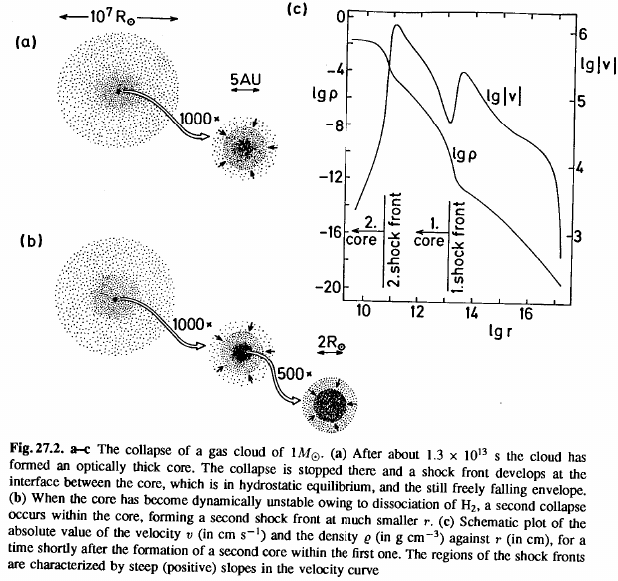
\includegraphics[trim={0cm 0cm 0cm 0cm},clip, keepaspectratio,width=0.8\textwidth]{collapsedensitystructure}\label{fig:collapsedensitystructure}
\end{figure}
\end{column}
\end{columns}
\end{frame}

\begin{frame}{core collapse}
\begin{columns}[T]
	\begin{column}{0.55\textwidth}
	\begin{itemize}
	\item For $H_2$ $\gamma_{ad}=\frac{f+2}{f}=\frac{7}{5}=1.4\approx\frac{4}{3}\approx1.33$, for $H$ $\gamma_{ad}=\frac{5}{3}\approx1.667$.  Slight decreases of $\gamma_{ad}<\frac{4}{3}$ by $H_2$ dissociation: collapse.
	\item When all hydrogen is dissociated $\gamma_{ad}>\frac{4}{3}$
	\item Central compression (of innermost core) is adiabatic as $\tau_{accr}<\tau_{KH}$, then $\dot{M}\to0$ and evolution is no more adiabatic.
	\end{itemize}
	\end{column}
	\begin{column}{0.45\textwidth}
	\begin{figure}[!ht]
	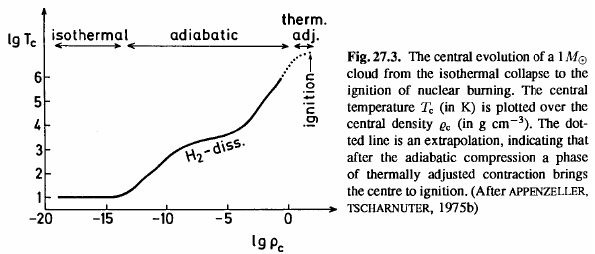
\includegraphics[trim={0cm 0cm 0cm 0cm},clip, keepaspectratio,width=0.99\textwidth]{centralcollapseevolution}\label{fig:centralcollapseevolution}
	\end{figure}
	\end{column}
\end{columns}
\end{frame}

\begin{frame}{Evolution of protostar in HR}
\begin{itemize}
\item Far from HE: radiation emitted by core is absorbed by envelope's grain and re-emitted in IR. Infalling envelope. Start on far right in HR diagram.
\item Thinning of envelope: photosphere moves downward until reaches core - $T_{ff}$ increases
\item In accretion phase $L\approx L_{accr}\propto\dot{M}$, then $L\approx L_g$ of core. Strong accretion rate heats core and make it isothermal, then a T gradient builds up and convection developes downward from surface - we found object on HL if fully convective, normal condition at border and envelope is thin in V.
\end{itemize}
\end{frame}

\subsection{Pre main sequence ed approccio a ZAMS per stelle di sequenza superiori/inferiori}\linkdest{preMS}

\begin{frame}{Traccia di Hayashi}
Primo/secondo core di Larson; Evoluzione di PMS sulla traccia di Hayashi; ruolo di opacit\'a di H- nella verticalit\'a della traccia di Hayashi; fusione deuterio; stelle completamente convettive o con nucleo radiativo. Abbondanza elementi leggeri in stelle di pre-sequenza
\end{frame}


\begin{frame}{Jeans mass ($\num{e5}\msun$)}
\todo{Instability} $\omega^2=k^2c_s^2-4\pi G\rho<0$:
\[\lambda>\lambda_H=\sqrt{\frac{\pi c_s^2}{G\rho}}=\SI{0.19}{\parsec}\sqrt{\frac{T}{\SI{10}{\kelvin}}}(\frac{n_{H^2}}{\SI{e4}{\per\cubic\cm}})\expy{-1/2}\]
\end{frame}

\begin{frame}{Protostar: first core and main accretion}
Virial T. $2E_i+\Omega=0$: $3kT\frac{M}{\mu m_H}=\int_0^M\frac{Gm}{r}\,dm$: collapse $\frac{3kTM}{\mu m_H}<\frac{3}{5}\frac{GM^2}{R}$ - $M>M_J=(\frac{3}{4\pi\rho})\expy{1/2}(\frac{5kT}{G\mu m_H})\expy{3/2}\propto T\expy{\frac{3}{2}}\rho\expy{-\frac{1}{2}}$
$t_{ff}\approx(G\rho)\expy{-\frac{1}{2}}\ll t_{cool}$: collasso adiabatico $P\propto T\expy{5/2}$ ($PT\expy{\frac{\gamma}{1-\gamma}}$) - $t_{ff}\gg t_{cool}$: collasso isotermo - \keyword{fragmentation}: Hydrostatic core surrounded by ff gas ($0.01\msun$) \todo{star formation hydrostatic core}
\end{frame}
